\documentclass[11pt,a4paper]{article}

% ── Pacotes ────────────────────────────────────────────────────────────────────
\usepackage[utf8]{inputenc}
\usepackage[T1]{fontenc}
\usepackage[provide=*,main=brazilian]{babel}
\usepackage{amsmath,amsthm,amssymb,amsfonts}
\usepackage{mathtools}
\usepackage{geometry}
\usepackage{graphicx}
\usepackage{float}
\usepackage{listings}
\usepackage{xcolor}
\usepackage{hyperref}
\usepackage{enumitem}
\usepackage{caption}
\usepackage{subcaption}
\usepackage{booktabs}
\usepackage{array}
\usepackage{tikz}
\usetikzlibrary{positioning, arrows.meta, shapes.geometric, calc}
\usepackage{pgfplots}
\pgfplotsset{compat=1.18}
\usepackage{tcolorbox}
\tcbuselibrary{theorems, skins, breakable}
\newfloat{algorithm}{H}{loa}
\floatname{algorithm}{Algoritmo}
\newenvironment{algorithmic}[1][0]{%
    \begin{list}{}{%
        \setlength{\leftmargin}{1.5em}%
        \setlength{\labelsep}{0pt}%
        \setlength{\itemsep}{0pt}%
        \setlength{\topsep}{0pt}%
        \setlength{\parsep}{0pt}%
        \setlength{\partopsep}{0pt}%
    }%
}{%
    \end{list}%
}
\newcommand{\State}{\item[]}
\newcommand{\Procedure}[2]{\item[\textbf{procedure} #1(#2)]}
\newcommand{\EndProcedure}{\item[\textbf{end procedure}]}
\newcommand{\If}[1]{\item[\textbf{if} #1 \textbf{then}]}
\newcommand{\Else}{\item[\textbf{else}]}
\newcommand{\EndIf}{\item[\textbf{end if}]}
\newcommand{\For}[1]{\item[\textbf{for} #1 \textbf{do}]}
\newcommand{\EndFor}{\item[\textbf{end for}]}
\newcommand{\Return}{\textbf{return}~}
\newcommand{\Call}[2]{\textsc{#1}(#2)}
\newcommand{\Comment}[1]{\hfill\textit{#1}}

% ── Configuração de página ─────────────────────────────────────────────────────
\geometry{margin=2.5cm, top=2.5cm, bottom=2.8cm}

% ── Hyperlinks ────────────────────────────────────────────────────────────────
\hypersetup{
    colorlinks=true,
    linkcolor=blue!60!black,
    citecolor=green!50!black,
    urlcolor=blue!70!black
}

% ── Ambientes de teoremas ──────────────────────────────────────────────────────
\theoremstyle{plain}
\newtheorem{theorem}{Teorema}[section]
\newtheorem{lemma}[theorem]{Lema}
\newtheorem{proposition}[theorem]{Proposição}
\newtheorem{corollary}[theorem]{Corolário}

\theoremstyle{definition}
\newtheorem{definition}[theorem]{Definição}
\newtheorem{remark}[theorem]{Observação}
\newtheorem{example}[theorem]{Exemplo}

% ── Caixas coloridas ───────────────────────────────────────────────────────────
\tcbset{
  motivacao/.style={
    colback=blue!5!white, colframe=blue!50!black,
    fonttitle=\bfseries, title=Motivação,
    breakable, enhanced
  },
  detalhe/.style={
    colback=green!5!white, colframe=green!40!black,
    fonttitle=\bfseries, title=Detalhe de Implementação,
    breakable, enhanced
  },
  atencao/.style={
    colback=orange!8!white, colframe=orange!60!black,
    fonttitle=\bfseries, title=Atenção,
    breakable, enhanced
  }
}

% ── Configuração de código ─────────────────────────────────────────────────────
\lstdefinestyle{jsstyle}{
    basicstyle=\ttfamily\footnotesize,
    keywordstyle=\color{blue!80!black}\bfseries,
    commentstyle=\color{gray!70!black}\itshape,
    stringstyle=\color{red!70!black},
    numbers=left,
    numberstyle=\tiny\color{gray},
    numbersep=8pt,
    breaklines=true,
    frame=single,
    rulecolor=\color{gray!30},
    backgroundcolor=\color{gray!4},
    tabsize=2,
    showstringspaces=false,
    morekeywords={let, const, class, constructor, of, async, await}
}
\lstset{style=jsstyle}

% ── Macros matemáticas ─────────────────────────────────────────────────────────
\newcommand{\R}{\mathbb{R}}
\newcommand{\N}{\mathbb{N}}
\newcommand{\vv}[1]{\mathbf{#1}}
\newcommand{\norm}[1]{\left\|#1\right\|}
\newcommand{\grad}{\nabla}
\newcommand{\eps}{\varepsilon}

% ── Título ─────────────────────────────────────────────────────────────────────
\title{%
  \textbf{Modelagem Geométrica: Representações Celulares,}\\[4pt]
  \textbf{Ray Tracing Volumétrico e Dinâmica de Partículas}\\[4pt]
  \textbf{em Tempo Real}\\[12pt]
  \large Motor de Cena 2D com Estruturas de Aceleração Espacial
}
\author{%
  Richard Elias Soares Viana\\
  Herivelton Siqueira\\
  \small IMPA Tech --- Graduação em Matemática Aplicada
}
\date{Maio de 2026}

% ──────────────────────────────────────────────────────────────────────────────
\begin{document}

\maketitle
\tableofcontents
\newpage

% ══════════════════════════════════════════════════════════════════════════════
\begin{abstract}
Este relatório detalha a concepção, a fundamentação matemática e a implementação
de um sistema interativo de modelagem geométrica bidimensional. O sistema integra
três pilares computacionais: \emph{(i)} representações celulares de formas
implícitas via grades uniformes e Quadtrees adaptativas; \emph{(ii)} um motor de
iluminação volumétrica baseado em \textit{Ray Tracing} acelerado por estrutura
espacial hierárquica; e \emph{(iii)} um sistema de partículas físicas com
colisões implícitas e cálculo de sombras em tempo real. Cada componente é
apresentado partindo da motivação matemática, passando pela dedução rigorosa dos
algoritmos e chegando até os detalhes concretos de implementação em JavaScript.
O objetivo central é demonstrar como conceitos de geometria diferencial, álgebra
linear e análise numérica se traduzem diretamente em código eficiente e
visualmente rico. Todo o conteudo produzido nesse projeto se encontra no github: \url{https://github.com/Heri-impatech/projeto-cg-impatech_oficial}.
\end{abstract}

\newpage

% ══════════════════════════════════════════════════════════════════════════════
\section{Introdução}

A representação de formas geométricas no computador é um problema que admite
abordagens radicalmente diferentes dependendo das operações que se deseja
realizar. Modelos paramétricos — como splines de Bézier ou NURBS — descrevem
a \emph{fronteira} de uma forma de maneira explícita e contínua, sendo naturais
para renderização e animação. No entanto, quando a pergunta central é
``\emph{um ponto $p$ está dentro ou fora desta forma?}'', os modelos
paramétricos exigem testes geométricos custosos.

As \textbf{superfícies implícitas} invertem essa lógica: uma forma é definida
pelo conjunto de zeros de uma função $f : \R^2 \to \R$,
\[
    \mathcal{S} = \{ (x, y) \in \R^2 \mid f(x, y) = 0 \},
\]
e o interior da forma é o conjunto $\{ f(x,y) \leq 0 \}$. Com isso, o teste de
inclusão de um ponto se reduz a avaliar $f$ naquele ponto --- uma operação de
tempo constante $O(1)$.

Este projeto explora como construir, sobre esse alicerce matemático, um sistema
computacional completo: discretizamos o espaço em células, construímos uma
hierarquia adaptativa (Quadtree), e usamos essa hierarquia para acelerar dois
sistemas físicos acoplados --- iluminação por \textit{Ray Tracing} e dinâmica de
partículas com colisões. O resultado é um ambiente interativo que roda em tempo
real no navegador, onde o usuário pode manipular as formas implícitas e observar
instantaneamente os efeitos sobre a luz e as partículas.

\subsection{Organização do Relatório}

O documento segue a mesma progressão lógica do código:

\begin{enumerate}[label=\S\arabic*.]
    \item \textbf{Funções Implícitas e o Problema de Inclusão} --- fundamentos
    matemáticos das formas utilizadas.
    \item \textbf{Discretização Celular e Classificação} --- como dividir o
    espaço em células e classificá-las em relação a uma forma.
    \item \textbf{Quadtrees Adaptativas} --- construção, subdivisão e poda da
    estrutura de aceleração espacial.
    \item \textbf{Ray Tracing Volumétrico} --- modelo de iluminação, travessia
    hierárquica e raymarching na fronteira.
    \item \textbf{Física de Partículas} --- integração de movimento, colisão
    implícita e sombras dinâmicas.
    \item \textbf{Integração do Sistema} --- como os módulos interagem no loop
    principal de renderização.
\end{enumerate}

% ══════════════════════════════════════════════════════════════════════════════
\section{Funções Implícitas e o Problema de Inclusão}
\label{sec:implicitas}

\subsection{Definição Formal}

\begin{definition}[Superfície Implícita 2D]
Seja $f : \Omega \subset \R^2 \to \R$ uma função contínua definida em um
domínio aberto $\Omega$. A \emph{superfície implícita} (ou curva implícita, em
duas dimensões) associada a $f$ é o conjunto de nível
\[
    \mathcal{S}_f = \{ (x, y) \in \Omega \mid f(x, y) = 0 \}.
\]
Além disso, definimos:
\begin{align*}
    \mathcal{I}_f &= \{ (x, y) \in \Omega \mid f(x, y) < 0 \} 
        && \text{(interior)} \\
    \mathcal{E}_f &= \{ (x, y) \in \Omega \mid f(x, y) > 0 \} 
        && \text{(exterior)}
\end{align*}
\end{definition}

A convenção de que o \emph{interior} corresponde a $f < 0$ é padrão em
geometria implícita e se alinha com a noção de que $f$ mede uma espécie de
``distância com sinal'' à superfície (embora não seja, em geral, a distância
euclideana).

\begin{tcolorbox}[motivacao]
Por que usar funções implícitas em vez de polígonos? Para um polígono com $n$
vértices, o teste clássico de ponto-interior (\textit{ray casting} ou
\textit{winding number}) tem complexidade $O(n)$. Para uma função implícita,
o teste é sempre $O(1)$: basta avaliar $f(p)$ e verificar o sinal. Isso é
fundamental para sistemas que precisam testar \emph{milhares} de pontos por
frame, como o nosso motor de física e iluminação.
\end{tcolorbox}

\subsection{Exemplos Concretos}

\paragraph{Círculo de centro $(c_x, c_y)$ e raio $r$:}
\[
    f(x, y) = (x - c_x)^2 + (y - c_y)^2 - r^2.
\]
O interior $f < 0$ é exatamente o disco aberto de raio $r$. Note que
$\grad f = 2(x - c_x, y - c_y)$, um vetor que aponta radialmente para fora do
centro --- o que será crucial para o cálculo de normais na física de partículas.

\paragraph{Parábola $y = x^2$ como fronteira:}
\[
    f(x, y) = y - x^2.
\]
O interior $f < 0$ é a região \emph{abaixo} da parábola, $\{y < x^2\}$.

\paragraph{Combinação de objetos (União Implícita):}
Dado um conjunto de formas $f_1, f_2, \ldots, f_k$, a função
\[
    f_{\text{union}}(x, y) = \min_i f_i(x, y)
\]
representa a \textbf{união} de todas as formas. Um ponto está dentro da união se
e somente se está dentro de \emph{ao menos uma} das formas, o que corresponde
exatamente a $\min_i f_i(p) \leq 0$. Esta é a operação implementada na classe
\texttt{Scene} do projeto:

\begin{lstlisting}
class Scene {
    evaluate(px, py) {
        let minVal = Infinity;
        for (let obj of this.objects)
            minVal = Math.min(minVal, obj.evaluate(px, py));
        return minVal;
    }
}
\end{lstlisting}

\subsection{Mapeamento de Coordenadas}
\label{subsec:coords}

O canvas do navegador usa um sistema de coordenadas em \emph{pixels}, com a
origem no canto superior esquerdo e o eixo $y$ apontando \emph{para baixo}. As
funções matemáticas clássicas, por outro lado, são naturalmente definidas em
coordenadas cartesianas com $y$ apontando para cima. O sistema realiza um
mapeamento afim bijetivo entre esses dois espaços.

Seja um canvas de largura $W$ e altura $H$ pixels. O domínio matemático escolhido
é $[-2, 2] \times [-2, 2]$. O mapeamento de pixel $(p_x, p_y)$ para coordenada
matemática $(x, y)$ é:
\begin{align}
    x &= -2 + p_x \cdot \frac{4}{W} \label{eq:mapx} \\
    y &= -2 + (H - p_y) \cdot \frac{4}{H} \label{eq:mapy}
\end{align}

O termo $(H - p_y)$ na equação~\eqref{eq:mapy} é responsável por inverter o eixo
$y$, convertendo a convenção ``$y$ cresce para baixo'' do canvas para a convenção
matemática ``$y$ cresce para cima''. A implementação direta aparece em
\texttt{geometry.js}:

\begin{lstlisting}
class CustomImplicit {
    constructor(canvasW, canvasH, exprStr) {
        this.scaleX = 4.0 / canvasW; // 4 = largura do dominio [-2,2]
        this.scaleY = 4.0 / canvasH;
        this.func = new Function('x', 'y', `return ${exprStr};`);
    }
    pxToDomainX(px) { return -2.0 + px * this.scaleX; }
    pxToDomainY(py) { return -2.0 + (this.canvasH - py) * this.scaleY; }
    evaluate(px, py) {
        return this.func(this.pxToDomainX(px), this.pxToDomainY(py));
    }
}
\end{lstlisting}

\begin{tcolorbox}[atencao]
O círculo interativo (adicionado com clique do mouse) usa uma escala diferente:
seu domínio é $[0,1] \times [0,1]$ em vez de $[-2,2] \times [-2,2]$, pois é
criado diretamente em coordenadas normalizadas de canvas. O raio padrão $r = 0.08$
corresponde a $8\%$ da largura do canvas.
\end{tcolorbox}

% ══════════════════════════════════════════════════════════════════════════════
\section{Discretização Celular e Classificação}
\label{sec:discretizacao}

\subsection{Motivação para a Discretização}

\begin{tcolorbox}[motivacao]
Funções implícitas são objetos contínuos e infinitamente detalhados. Para
\emph{renderizá-las} e \emph{consultar} se um raio as atravessa, precisamos de
uma representação finita e discreta. A ideia de discretizar o espaço em células
é análoga à integração numérica: substituímos um objeto contínuo por uma
aproximação em malha, com resolução controlável. A chave é que, mesmo que uma
célula não seja pequena o suficiente para capturar a fronteira exatamente, ela
pode ser \emph{classificada} de forma conservadora --- o que é suficiente para
a aceleração espacial.
\end{tcolorbox}

\subsection{Grade Uniforme}

A abordagem mais simples consiste em dividir o domínio $[0, W] \times [0, H]$
em uma grade regular de $n \times n$ células, cada uma com dimensões
$\Delta x = W/n$ e $\Delta y = H/n$. A célula na posição $(i, j)$ ocupa a
região
\[
    C_{ij} = [i \Delta x,\; (i+1)\Delta x] \times [j \Delta y,\; (j+1)\Delta y].
\]

\subsubsection{Classificação de Células}

O \textbf{status} de uma célula descreve sua relação com a forma implícita:

\begin{center}
\begin{tabular}{clll}
\toprule
\textbf{Status} & \textbf{Nome} & \textbf{Cor} & \textbf{Significado} \\
\midrule
0 & Exterior & Branco & $f > 0$ em toda a célula \\
1 & Interior & Azul   & $f \leq 0$ em toda a célula \\
2 & Fronteira & Vermelho & $f$ muda de sinal na célula \\
\bottomrule
\end{tabular}
\end{center}

A determinação rigorosa do status exigiria verificar $f$ em \emph{todos} os
pontos da célula --- um problema inviável. Na prática, usamos uma
\textbf{heurística de amostragem} nos 4 cantos e no centro da célula:

\begin{definition}[Classificação por Amostragem]
Seja $P = \{ (x_{\min}, y_{\min}),\; (x_{\max}, y_{\min}),\; (x_{\max}, y_{\max}),\; (x_{\min}, y_{\max}),\; (x_c, y_c) \}$ o conjunto dos 4 cantos e do centro de uma célula. Definimos:
\[
    k = \#\{ p \in P \mid f(p) \leq 0 \}.
\]
Então:
\[
    \text{status}(C) = \begin{cases}
        1 & \text{se } k = 5 \text{ (todos dentro)} \\
        0 & \text{se } k = 0 \text{ (todos fora)} \\
        2 & \text{caso contrário (fronteira estimada)}
    \end{cases}
\]
\end{definition}

\begin{remark}
Esta heurística pode errar em casos extremos: uma forma muito pequena que toque
o interior de uma célula sem passar por nenhum dos 5 pontos amostrados seria
classificada como Status 0 (exterior), quando na verdade deveria ser Status 2.
Na prática, para formas suaves e resoluções razoáveis de grade, isso não é um
problema. Para círculos, existe uma classificação \emph{exata} baseada na
distância do centro ao retângulo mais próximo, que é implementada na classe
\texttt{Circle} (ver Seção~\ref{subsec:circle_exact}).
\end{remark}

\subsection{Classificação Exata para Círculos}
\label{subsec:circle_exact}

Para o círculo de centro $(c_x, c_y)$ e raio $r$, é possível determinar o status
de uma célula de forma \emph{exata} sem recorrer a amostragem. A ideia é calcular
a distância mínima do centro do círculo ao retângulo (célula).

\begin{proposition}[Classificação Exata do Círculo]
Seja $C$ uma célula com limites $[x_{\min}, x_{\max}] \times [y_{\min}, y_{\max}]$.
O ponto do retângulo $C$ mais próximo do centro $(c_x, c_y)$ é
\[
    q = \bigl(\operatorname{clamp}(c_x, x_{\min}, x_{\max}),\;
              \operatorname{clamp}(c_y, y_{\min}, y_{\max})\bigr),
\]
onde $\operatorname{clamp}(v, a, b) = \max(a, \min(b, v))$.

Então:
\begin{enumerate}
    \item Se $\norm{q - (c_x, c_y)}^2 > r^2$: a célula é \textbf{exterior} (Status 0). O círculo não alcança a célula.
    \item Se todos os 4 cantos satisfazem $(p_x - c_x)^2 + (p_y - c_y)^2 < r^2$: a célula é \textbf{interior} (Status 1).
    \item Caso contrário: a célula é \textbf{fronteira} (Status 2).
\end{enumerate}
\end{proposition}

\begin{proof}
(1) Se o ponto mais próximo do retângulo ao centro $c$ está fora do círculo, então
todo o retângulo está fora, pois todos os demais pontos do retângulo estão ainda
mais distantes de $c$.

(2) Se todos os cantos estão dentro do círculo e o raio do círculo é maior que
a distância de $c$ ao retângulo, então, como os cantos são os extremos do
retângulo convexo, todos os pontos intermediários também estão dentro.

(3) É um caso misto: o círculo intercepta, mas não contém completamente o
retângulo.
\end{proof}

A implementação em JavaScript:
\begin{lstlisting}
classifyCell(xMinPx, xMaxPx, yMinPx, yMaxPx) {
    // Converte para coordenadas de dominio (normalizado 0..1)
    const xMin = this.pxToDomainX(xMinPx), xMax = this.pxToDomainX(xMaxPx);
    const yMin = this.pxToDomainY(yMaxPx), yMax = this.pxToDomainY(yMinPx);

    // Passo 1: ponto mais proximo do centro no retangulo
    const closestX = clamp(this.cx, xMin, xMax);
    const closestY = clamp(this.cy, yMin, yMax);
    const dx = closestX - this.cx, dy = closestY - this.cy;

    // Se o ponto mais proximo esta fora do circulo => Status 0
    if (dx*dx + dy*dy > this.rSq) return 0;

    // Verifica se TODOS os cantos estao dentro
    const corners = [[xMin,yMin],[xMax,yMin],[xMax,yMax],[xMin,yMax]];
    for (let c of corners)
        if ((c[0]-this.cx)**2 + (c[1]-this.cy)**2 >= this.rSq) return 2;

    return 1; // Todos os cantos dentro => Status 1
}
\end{lstlisting}

% ══════════════════════════════════════════════════════════════════════════════
\section{Quadtree Adaptativa}
\label{sec:quadtree}

\subsection{Motivação para a Adaptatividade}

\begin{tcolorbox}[motivacao]
Uma grade uniforme de resolução $n$ possui $n^2$ células. Para $n = 512$ (o que
daria fronteiras com precisão de 1 pixel em um canvas de 512px), teríamos
$262.144$ células. A maioria estaria classificada como Status 0 (exterior) ou
Status 1 (interior) --- informação quase inútil para o Ray Tracer, que só
precisa saber \emph{onde estão as fronteiras}. A Quadtree resolve isso: ela
refina \emph{somente} as células de fronteira (Status 2), concentrando o poder
computacional onde ele importa. Células claramente interiores ou exteriores são
representadas por um único nó, independentemente de seu tamanho.
\end{tcolorbox}

\subsection{Definição Recursiva}

\begin{definition}[Quadtree]
Uma Quadtree sobre uma região retangular $R$ e uma forma implícita $f$ é uma
árvore quaternária definida recursivamente:
\begin{itemize}
    \item A \emph{raiz} representa a região $R$ inteira.
    \item Se um nó $v$ (representando a sub-região $R_v$) tem Status 2 e a
    profundidade de $v$ é menor que $d_{\max}$, ele é \emph{subdividido}: $R_v$
    é particionada em quatro quadrantes iguais $R_{v,1}, R_{v,2}, R_{v,3}, R_{v,4}$,
    que se tornam os quatro filhos de $v$.
    \item Nós com Status 0 ou Status 1, ou nós em profundidade $d_{\max}$, são
    \emph{folhas}.
\end{itemize}
\end{definition}

\begin{figure}[H]
\centering
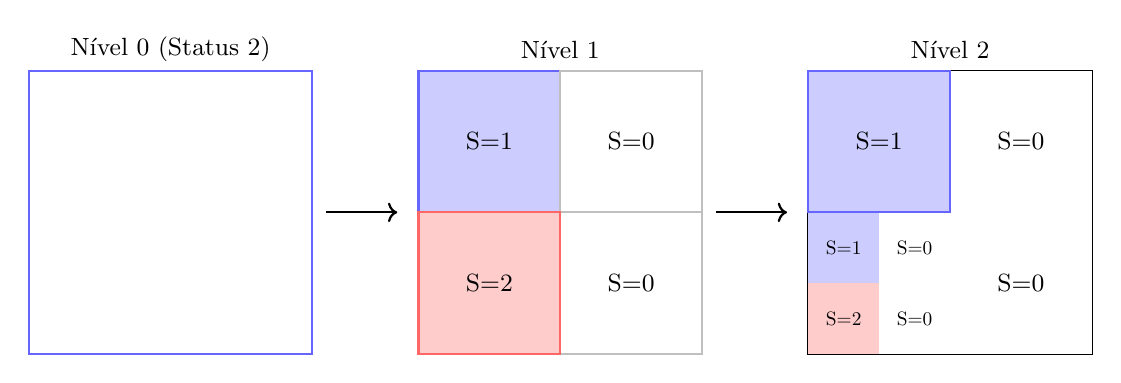
\begin{tikzpicture}[scale=0.9]
  % Nivel 0: quadrado completo
  \draw[thick, blue!60] (0,0) rectangle (4,4);
  \node at (2,4.3) {\small Nível 0 (Status 2)};

  % Nivel 1: quatro quadrantes
  \begin{scope}[xshift=5.5cm]
    \draw[thick] (0,0) rectangle (4,4);
    \draw[dashed, gray] (2,0)--(2,4);
    \draw[dashed, gray] (0,2)--(4,2);
    % Status dos quadrantes
    \fill[blue!20] (0,2) rectangle (2,4);   \node at (1,3) {\small S=1};
    \fill[white]   (2,2) rectangle (4,4);   \node at (3,3) {\small S=0};
    \fill[white]   (2,0) rectangle (4,2);   \node at (3,1) {\small S=0};
    \fill[red!20]  (0,0) rectangle (2,2);   \node at (1,1) {\small S=2};
    \draw[thick, blue!60] (0,2) rectangle (2,4);
    \draw[thick, gray!50] (2,2) rectangle (4,4);
    \draw[thick, gray!50] (2,0) rectangle (4,2);
    \draw[thick, red!60] (0,0) rectangle (2,2);
    \node at (2,4.3) {\small Nível 1};
  \end{scope}

  % Nivel 2: subdivisao do quadrante S=2
  \begin{scope}[xshift=11cm]
    \draw[thick] (0,0) rectangle (4,4);
    \draw[dashed, gray] (2,0)--(2,4);
    \draw[dashed, gray] (0,2)--(4,2);
    \fill[blue!20] (0,2) rectangle (2,4);   \node at (1,3) {\small S=1};
    \fill[white]   (2,2) rectangle (4,4);   \node at (3,3) {\small S=0};
    \fill[white]   (2,0) rectangle (4,2);   \node at (3,1) {\small S=0};
    % Subdivisao do quadrante inferior esquerdo
    \draw[dashed, red!50] (1,0)--(1,2);
    \draw[dashed, red!50] (0,1)--(2,1);
    \fill[blue!20]  (0,1) rectangle (1,2);  \node[scale=0.7] at (0.5,1.5) {S=1};
    \fill[white]    (1,1) rectangle (2,2);  \node[scale=0.7] at (1.5,1.5) {S=0};
    \fill[red!20]   (0,0) rectangle (1,1);  \node[scale=0.7] at (0.5,0.5) {S=2};
    \fill[white]    (1,0) rectangle (2,1);  \node[scale=0.7] at (1.5,0.5) {S=0};
    \draw[thick, blue!60] (0,2) rectangle (2,4);
    \node at (2,4.3) {\small Nível 2};
  \end{scope}

  % Setas entre niveis
  \draw[->, thick] (4.2,2) -- (5.2,2);
  \draw[->, thick] (9.7,2) -- (10.7,2);
\end{tikzpicture}
\caption{Construção iterativa da Quadtree. Apenas células com Status 2 (vermelho)
são subdivididas. Células com Status 0 (branco) ou Status 1 (azul) são folhas.}
\label{fig:quadtree_build}
\end{figure}

\subsection{Algoritmo de Construção}

O algoritmo de construção é uma busca em profundidade (\textit{DFS}) que
constrói a árvore top-down:

\begin{algorithm}[H]
\caption{Construção da Quadtree}
\begin{algorithmic}[1]
\Procedure{Build}{$R$, $d$, $d_{\max}$, $f$}
    \State $s \gets \text{ClassifyCell}(R, f)$
    \State $v \gets \text{NovoNó}(R, s)$
    \If{$s = 2$ \textbf{and} $d < d_{\max}$}
        \State $(R_1, R_2, R_3, R_4) \gets \text{Subdividir}(R)$
        \For{$i = 1, 2, 3, 4$}
            \State $v.\text{filhos}[i] \gets \Call{Build}{R_i, d+1, d_{\max}, f}$
        \EndFor
    \EndIf
    \State \Return $v$
\EndProcedure
\end{algorithmic}
\end{algorithm}

A subdivisão de um nó com região $[x_{\min}, x_{\max}] \times [y_{\min}, y_{\max}]$
produz quatro filhos:
\begin{align*}
    R_1 &= [x_{\min},\; x_c] \times [y_{\min},\; y_c]
        & (\text{inferior esquerdo}) \\
    R_2 &= [x_c,\; x_{\max}] \times [y_{\min},\; y_c]
        & (\text{inferior direito}) \\
    R_3 &= [x_c,\; x_{\max}] \times [y_c,\; y_{\max}]
        & (\text{superior direito}) \\
    R_4 &= [x_{\min},\; x_c] \times [y_c,\; y_{\max}]
        & (\text{superior esquerdo})
\end{align*}
onde $x_c = (x_{\min} + x_{\max})/2$ e $y_c = (y_{\min} + y_{\max})/2$.

\subsubsection{Complexidade}

\begin{proposition}[Complexidade da Quadtree]
Seja $L$ o número de células de fronteira (Status 2) na resolução máxima
$d_{\max}$. Então a Quadtree tem $O(L \cdot d_{\max})$ nós no total.
\end{proposition}

Na prática, para uma curva suave, $L = O(W \cdot H / 2^{d_{\max}})$ cresce
linearmente com o perímetro discreto, e a Quadtree representa a fronteira com
muito menos memória do que uma grade uniforme de resolução equivalente.

\subsection{Poda (Pruning)}
\label{subsec:pruning}

\begin{tcolorbox}[motivacao]
A poda pós-construção tem dois objetivos: \emph{(i)} reduzir o uso de memória
eliminando subdivisões desnecessárias; e \emph{(ii)} acelerar a travessia de
raios. No Ray Tracing, quando um raio entra em um nó folha com Status 0 (vazio),
podemos imediatamente descartá-lo sem processar filhos. A poda garante que não
existam nós com filhos redundantes --- um nó pai com quatro filhos todos do
mesmo status é equivalente a uma única folha daquele status.
\end{tcolorbox}

\begin{definition}[Poda de Quadtree]
Dado um nó $v$ com filhos $v_1, v_2, v_3, v_4$, se
$\text{status}(v_1) = \text{status}(v_2) = \text{status}(v_3) = \text{status}(v_4) = s$
para algum $s \in \{0, 1\}$, então descartamos os filhos e definimos
$\text{status}(v) \gets s$. O nó $v$ se torna uma folha.
\end{definition}

O algoritmo de poda é um percurso em pós-ordem (\textit{post-order DFS}):
primeiro processamos todos os filhos recursivamente, depois verificamos se o nó
pai pode ser podado.

\begin{algorithm}[H]
\caption{Poda da Quadtree (post-order)}
\begin{algorithmic}[1]
\Procedure{Prune}{$v$}
    \If{$v$ é folha} \Return \EndIf
    \For{cada filho $c$ de $v$}
        \State \Call{Prune}{$c$}
    \EndFor
    \State $s_0 \gets \text{status}(v.\text{filho}_1)$
    \If{todos os filhos têm o mesmo status $s_0$ \textbf{and} $s_0 \neq 2$}
        \State $v.\text{filhos} \gets \emptyset$ \Comment{descarta os filhos}
        \State $v.\text{status} \gets s_0$    \Comment{v vira folha}
    \EndIf
\EndProcedure
\end{algorithmic}
\end{algorithm}

\begin{remark}
A poda só é aplicada para Status 0 e 1, nunca para Status 2. Um nó com quatro
filhos de fronteira (Status 2) \emph{não} pode ser fundido, pois isso perderia
informação sobre onde a fronteira está localizada dentro de cada filho.
\end{remark}

% ══════════════════════════════════════════════════════════════════════════════
\section{Ray Tracing Volumétrico}
\label{sec:raytracing}

\subsection{Modelo de Iluminação e Motivação}

\begin{tcolorbox}[motivacao]
Um renderizador baseado em \emph{ray casting} simples lançaria um raio de cada
pixel até a cena, determinando sua cor. Aqui invertemos a lógica: lançamos raios
\emph{a partir da fonte de luz} em todas as direções. Cada raio carrega a luz
da lanterna até encontrar uma parede (fronteira da forma implícita) ou atingir
o limite de alcance. Os pixels iluminados por pelo menos um raio ficam visíveis;
os demais permanecem no escuro. Isso é eficiente para simular uma única fonte
de luz direcional com sombras corretas.
\end{tcolorbox}

\subsection{Equação do Raio}

Um raio é parametrizado por:
\[
    \vv{r}(t) = \vv{o} + t \vv{d}, \quad t \geq 0,
\]
onde $\vv{o} = (o_x, o_y)$ é a origem (posição da lanterna) e
$\vv{d} = (d_x, d_y)$ é o vetor direção unitário ($\norm{\vv{d}} = 1$). Para
cada ângulo $\theta_i = i \cdot \frac{2\pi}{N_{\text{raios}}}$, lançamos um raio
com direção
\[
    \vv{d}_i = (\cos\theta_i,\; \sin\theta_i).
\]

\subsection{Interseção Raio--AABB: O Método das Lâminas}
\label{subsec:aabb}

Para percorrer a Quadtree eficientemente, precisamos determinar se um raio
intersecta um nó (uma caixa delimitadora alinhada aos eixos, AABB). O método
das lâminas (\textit{slab method}) resolve isso de forma eficiente.

\begin{definition}[AABB]
Uma AABB em 2D é um retângulo alinhado aos eixos:
$B = [x_{\min}, x_{\max}] \times [y_{\min}, y_{\max}]$.
\end{definition}

\begin{theorem}[Interseção Raio-AABB]
O raio $\vv{r}(t) = \vv{o} + t\vv{d}$ intersecta a AABB $B$ se e somente se
o intervalo de interseção $[t_{\min}, t_{\max}]$, definido como abaixo, satisfaz
$t_{\max} \geq t_{\min}$ e $t_{\max} \geq 0$.
\end{theorem}

\begin{proof}
Para cada eixo $k \in \{x, y\}$, o raio está dentro da ``lâmina''
$[B_{k,\min}, B_{k,\max}]$ para $t \in [t_{k,1}, t_{k,2}]$, onde
\[
    t_{k,1} = \frac{B_{k,\min} - o_k}{d_k}, \qquad
    t_{k,2} = \frac{B_{k,\max} - o_k}{d_k}.
\]
(Se $d_k = 0$, o raio é paralelo ao eixo: está dentro da lâmina se e somente se
$o_k \in [B_{k,\min}, B_{k,\max}]$, caso contrário não há interseção.)

O raio está \emph{simultaneamente} dentro de todas as lâminas para
$t \in [t_{\min}, t_{\max}]$, onde
\[
    t_{\min} = \max_k \min(t_{k,1}, t_{k,2}), \qquad
    t_{\max} = \min_k \max(t_{k,1}, t_{k,2}).
\]
A condição $t_{\max} \geq t_{\min}$ garante que este intervalo é não-vazio (o
raio está em todas as lâminas ao mesmo tempo). A condição $t_{\max} \geq 0$
garante que a interseção ocorre à frente da origem.
\end{proof}

A implementação direta:
\begin{lstlisting}
rayIntersectAABB(ox, oy, dx, dy, xMin, yMin, xMax, yMax) {
    let tmin = -Infinity, tmax = Infinity;

    // Lamina do eixo X
    if (Math.abs(dx) > 1e-6) {
        let tx1 = (xMin - ox) / dx;
        let tx2 = (xMax - ox) / dx;
        tmin = Math.max(tmin, Math.min(tx1, tx2));
        tmax = Math.min(tmax, Math.max(tx1, tx2));
    } else if (ox < xMin || ox > xMax) return null; // Paralelo e fora

    // Lamina do eixo Y
    if (Math.abs(dy) > 1e-6) {
        let ty1 = (yMin - oy) / dy;
        let ty2 = (yMax - oy) / dy;
        tmin = Math.max(tmin, Math.min(ty1, ty2));
        tmax = Math.min(tmax, Math.max(ty1, ty2));
    } else if (oy < yMin || oy > yMax) return null;

    if (tmax >= tmin && tmax >= 0)
        return { tmin: Math.max(0, tmin), tmax };
    return null;
}
\end{lstlisting}

\subsection{Travessia Hierárquica da Quadtree}
\label{subsec:traversal}

Com o teste de interseção raio-AABB em mãos, podemos percorrer a Quadtree de
forma eficiente. A ideia central é a \textbf{poda por visibilidade}: se um raio
não intersecta a AABB de um nó, ele não pode intersectar nenhum descendente
daquele nó, pois as AABBs dos filhos estão contidas na do pai.

Além disso, exploramos o conhecimento sobre o \textbf{estado da luz}: se a
lanterna está \emph{fora} dos objetos ($f(\vv{o}) > 0$), os raios viajam
livremente pelo exterior (Status 0) e só colidem ao tentar entrar em uma forma
($f \leq 0$). Portanto, podemos \textbf{ignorar completamente} nós com Status 0.
Simetricamente, se a luz está \emph{dentro}, ignoramos nós com Status 1.

\begin{algorithm}[H]
\caption{Travessia de Raio na Quadtree}
\begin{algorithmic}[1]
\Procedure{Trace}{$v$, $\vv{o}$, $\vv{d}$, isInside, scene}
    \If{$v$ é nulo} \Return \textbf{null} \EndIf
    \If{isInside \textbf{and} $v.\text{status} = 1$} \Return \textbf{null} \EndIf
    \Comment{Luz viaja livre no interior}
    \If{\textbf{not} isInside \textbf{and} $v.\text{status} = 0$} \Return \textbf{null} \EndIf
    \Comment{Luz viaja livre no exterior}
    \If{Raio não intersecta AABB de $v$} \Return \textbf{null} \EndIf
    \If{$v$ tem filhos}
        \State Calcula $t_{\min}$ de interseção de cada filho com o raio
        \State Ordena filhos por $t_{\min}$ crescente \Comment{Nearest-first}
        \For{cada filho $c$ em ordem}
            \State resultado $\gets$ \Call{Trace}{$c$, $\vv{o}$, $\vv{d}$, isInside, scene}
            \If{resultado $\neq$ \textbf{null}} \Return resultado \EndIf
        \EndFor
        \Return \textbf{null}
    \Else \Comment{Nó folha de fronteira: raymarching fino}
        \State \Return \Call{Raymarch}{$v$, $\vv{o}$, $\vv{d}$, isInside, scene}
    \EndIf
\EndProcedure
\end{algorithmic}
\end{algorithm}

\begin{tcolorbox}[detalhe]
\textbf{Por que ordenar os filhos por $t_{\min}$?} Na travessia, assim que
encontramos a \emph{primeira} colisão, podemos retornar imediatamente
(\textit{early exit}). Visitando os filhos em ordem crescente de $t_{\min}$
(da esquerda para a direita ao longo do raio), garantimos que a primeira colisão
encontrada é de fato a mais próxima da origem. Sem essa ordenação, poderíamos
reportar uma colisão mais distante antes de uma mais próxima, produzindo sombras
incorretas.
\end{tcolorbox}

\subsection{Raymarching na Fronteira}
\label{subsec:raymarch}

Ao atingir um nó folha com Status 2 (fronteira), não temos a equação analítica
da interseção raio--forma. A solução é o \textbf{raymarching}: amostramos a
função $f$ em passos discretos ao longo do raio e detectamos a mudança de sinal.

Para um nó com intervalo de interseção $[t_{\min}, t_{\max}]$, iteramos:
\[
    t_k = t_{\min} + k \cdot \Delta t, \quad k = 0, 1, 2, \ldots
\]
e avaliamos $f(\vv{r}(t_k)) = f(o_x + d_x t_k,\; o_y + d_y t_k)$.

A colisão é detectada por uma \emph{mudança de sinal} que depende do estado:
\begin{align*}
    \text{(luz fora):} & \quad f(\vv{r}(t_k)) \leq 0 
        \Rightarrow \text{hit em } t_k \\
    \text{(luz dentro):} & \quad f(\vv{r}(t_k)) > 0
        \Rightarrow \text{hit em } t_k
\end{align*}

O passo $\Delta t = 1.0$ pixel foi escolhido para que nenhuma fronteira seja
``pulada'' --- como a fronteira tem, no mínimo, 1 pixel de espessura na
resolução do canvas, um passo de 1 pixel garante que ela será detectada.

\begin{remark}
O raymarching é executado \emph{somente dentro de nós folha de Status 2}. O
resto da árvore é percorrido analiticamente pelo teste AABB. Isso é a essência
da aceleração: trocamos o teste analítico barato (AABB) pelo teste caro
(avaliação de $f$) apenas onde é absolutamente necessário.
\end{remark}

\subsection{Detecção de Imersão e Iluminação Invertida}
\label{subsec:imersao}

Um recurso elegante do sistema é o suporte a uma lanterna dentro de um objeto.
O estado de imersão é determinado avaliando a cena na posição da lanterna:
\[
    \text{isInside} = \bigl( f_{\text{scene}}(o_x, o_y) \leq 0 \bigr).
\]

Quando \texttt{isInside = true}:
\begin{itemize}
    \item A cor base dos raios muda de amarela $(255, 245, 220)$ para azul $(74, 144, 217)$.
    \item O raio viaja pelo interior (azul na Quadtree) sem obstrução.
    \item A colisão ocorre quando o raio \emph{tenta sair} do objeto ($f > 0$).
    \item O resultado visual é que o interior do objeto é iluminado, enquanto o
    exterior permanece no escuro --- como uma luz dentro de uma bolha de vidro.
\end{itemize}

\subsection{Modelo de Decaimento de Luz}
\label{subsec:decaimento}

A intensidade da luz decai com a distância. Usamos uma função de decaimento
\textbf{polinomial} de expoente $\alpha = 2.5$:
\[
    I(t) = I_0 \cdot \left(1 - \frac{t}{R}\right)^\alpha, \quad 0 \leq t \leq R,
\]
onde $R$ é o alcance máximo da lanterna (parâmetro \texttt{lightRange}) e $I_0$
é a intensidade na origem.

\begin{tcolorbox}[motivacao]
Por que $\alpha = 2.5$ em vez do decaimento quadrático inverso da lei física
$I \propto 1/t^2$? A lei $1/t^2$ produz um pico extremamente brilhante próximo
à origem e escuridão abrupta à distância, o que é visualmente agressivo em tempo
real. A função $(1 - t/R)^{2.5}$ garante que $I(R) = 0$ (a luz se apaga suavemente
no limite do alcance), produz um núcleo brilhante e uma queda gradual que o olho
humano percebe como ``natural''. O expoente $2.5$ foi escolhido empiricamente
como um bom compromisso entre brilho central e suavidade nas bordas.
\end{tcolorbox}

Para renderizar o gradiente, o sistema cria um gradiente linear do Canvas 2D da
origem até o ponto final do raio, com quatro paradas:

\begin{center}
\begin{tabular}{cll}
\toprule
\textbf{Posição} & \textbf{Opacidade} & \textbf{Correspondência à fórmula} \\
\midrule
$t/R = 0$    & $1.0$  & $I(0) = I_0$ \\
$t/R = 0.15$ & $0.8$  & $I(0.15R) \approx 0.75 I_0$ \\
$t/R = 0.5$  & $0.25$ & $I(0.5R) \approx 0.18 I_0$ \\
$t/R = 1.0$  & $0.0$  & $I(R) = 0$ \\
\bottomrule
\end{tabular}
\end{center}

\subsection{Visualização do Modo Adaptativo}

No modo de visualização ``Estrutura Quadtree'', o sistema usa o
\texttt{AdaptiveQuadtreeAnimator} para revelar progressivamente a estrutura da
árvore, pintando cada nó com a cor correspondente ao seu status. A revelação
segue uma travessia BFS (largura), tornando visível a progressão hierárquica do
nível raiz até as folhas mais refinadas.

A animação funciona mantendo uma \texttt{ImageData} (buffer de pixels bruto)
que é atualizada incrementalmente a cada frame. O método \texttt{step(nowMs)}
calcula quantos nós revelar com base no tempo decorrido, garantindo que a
velocidade de revelação seja independente da taxa de frames:
\[
    \Delta n = \left\lfloor \frac{\Delta t_{\text{elapsed}}}{\Delta t_{\text{step}}} \right\rfloor,
\]
onde $\Delta t_{\text{step}}$ é o intervalo mínimo entre revelações (30ms
no sistema atual).

% ══════════════════════════════════════════════════════════════════════════════
\section{Física de Partículas e Colisões Implícitas}
\label{sec:particulas}

\subsection{Modelo de Movimento}

Cada partícula é um ponto com posição $\vv{p} = (x, y)$ e velocidade
$\vv{v} = (v_x, v_y)$. A integração de Euler explícita atualiza o estado a
cada frame:
\[
    \vv{p}^{(n+1)} = \vv{p}^{(n)} + \Delta t \cdot \vv{v}^{(n)},
\]
onde o passo de tempo $\Delta t$ é implicitamente 1 frame (a velocidade é
expressa em pixels/frame).

As paredes do canvas são tratadas como bordas rígidas: ao ultrapassar qualquer
borda, a componente correspondente da velocidade é invertida.

\subsection{Colisão com Formas Implícitas: Reflexão Pelo Gradiente}

\begin{tcolorbox}[motivacao]
Como fazer uma partícula ``quicar'' numa forma implícita arbitrária, sem conhecer
sua geometria explicitamente? O gradiente $\grad f$ aponta na direção de maior
crescimento de $f$, que é perpendicular à curva $f = 0$. Portanto,
$\hat{\vv{n}} = \grad f / \norm{\grad f}$ é a \textbf{normal} à superfície
implícita. Com a normal, podemos aplicar a lei clássica de reflexão especular
para calcular o novo vetor velocidade após a colisão.
\end{tcolorbox}

Quando a posição tentativa $\vv{p}^* = \vv{p} + \vv{v}$ cai dentro de uma
forma ($f(\vv{p}^*) \leq 0$), a colisão é detectada. O gradiente é aproximado
por diferenças finitas centrais com passo $\eps = 1.0$ pixel:
\begin{align}
    \frac{\partial f}{\partial x}(\vv{p}^*) &\approx
        \frac{f(p^*_x + \eps,\; p^*_y) - f(p^*_x - \eps,\; p^*_y)}{2\eps}
        \label{eq:grad_x} \\
    \frac{\partial f}{\partial y}(\vv{p}^*) &\approx
        \frac{f(p^*_x,\; p^*_y + \eps) - f(p^*_x,\; p^*_y - \eps)}{2\eps}
        \label{eq:grad_y}
\end{align}

Como $\eps$ é constante e cancela na normalização do vetor, simplificamos
calculando apenas o numerador:
\[
    \vv{g} = \bigl(f(p^*_x + \eps, p^*_y) - f(p^*_x - \eps, p^*_y),\;
                   f(p^*_x, p^*_y + \eps) - f(p^*_x, p^*_y - \eps)\bigr).
\]

A normal unitária é $\hat{\vv{n}} = \vv{g} / \norm{\vv{g}}$. A velocidade
refletida é dada pela fórmula de reflexão especular:
\begin{equation}
    \label{eq:reflexao}
    \vv{v}' = \vv{v} - 2 (\vv{v} \cdot \hat{\vv{n}}) \hat{\vv{n}}.
\end{equation}

\begin{proof}[Dedução da Fórmula de Reflexão]
Decompomos $\vv{v}$ em componentes normal e tangencial à superfície:
\[
    \vv{v} = \underbrace{(\vv{v} \cdot \hat{\vv{n}}) \hat{\vv{n}}}_{\vv{v}_n}
             + \underbrace{(\vv{v} - (\vv{v} \cdot \hat{\vv{n}})\hat{\vv{n}})}_{\vv{v}_t}.
\]
Na reflexão elástica, a componente tangencial é preservada e a componente normal
é invertida: $\vv{v}'_n = -\vv{v}_n$, $\vv{v}'_t = \vv{v}_t$. Portanto:
\[
    \vv{v}' = \vv{v}_t + \vv{v}'_n = \vv{v}_t - \vv{v}_n
            = \vv{v} - 2\vv{v}_n
            = \vv{v} - 2(\vv{v} \cdot \hat{\vv{n}})\hat{\vv{n}}.
\]
\end{proof}

A implementação em JavaScript:
\begin{lstlisting}
update(scene, w, h) {
    let nextX = this.x + this.vx;
    let nextY = this.y + this.vy;

    if (scene.evaluate(nextX, nextY) <= 0) {
        const eps = 1.0;
        // Gradiente por diferencas finitas (eq. 6.3 e 6.4)
        const nx = scene.evaluate(nextX+eps, nextY) 
                 - scene.evaluate(nextX-eps, nextY);
        const ny = scene.evaluate(nextX, nextY+eps) 
                 - scene.evaluate(nextX, nextY-eps);
        const len = Math.sqrt(nx*nx + ny*ny) || 1; // ||grad f||

        // Formula de reflexao (eq. 6.5)
        const dot = (this.vx*nx + this.vy*ny) / len;
        this.vx -= 2 * dot * (nx / len);
        this.vy -= 2 * dot * (ny / len);
        // Nao avanca a posicao (permanece fora da forma)
    } else {
        this.x = nextX;
        this.y = nextY;
    }
}
\end{lstlisting}

\subsection{Sombras Dinâmicas por Shadow Ray}
\label{subsec:shadowray}

Para cada partícula visível, verificamos se ela está na ``linha de visão'' da
lanterna. Isso é feito lançando um \textbf{shadow ray} da lanterna em direção
à partícula.

Seja $\vv{o}$ a posição da lanterna, $\vv{p}$ a posição da partícula e
$d_{\vv{op}} = \norm{\vv{p} - \vv{o}}$ a distância entre elas. O shadow ray
tem direção
\[
    \hat{\vv{d}} = \frac{\vv{p} - \vv{o}}{d_{\vv{op}}}.
\]

A partícula está em sombra se e somente se o ray tracer detecta uma colisão a
uma distância $t_{\text{hit}} < d_{\vv{op}} - r_{\text{partícula}}$ --- a
subtração de $r_{\text{partícula}}$ evita que a partícula faça sombra sobre si
mesma (\textit{self-shadowing}).

Se a partícula não está em sombra, sua opacidade visual é modulada pelo mesmo
modelo de decaimento da Seção~\ref{subsec:decaimento}:
\[
    \alpha_{\text{halo}} = \left(1 - \frac{d_{\vv{op}}}{R}\right)^{2.5},
\]
criando um efeito de ``partícula dentro do cone de luz''.

% ══════════════════════════════════════════════════════════════════════════════
\section{Análise de Complexidade e Performance}
\label{sec:complexidade}

\subsection{Custo do Ray Tracing por Frame}

Seja $N$ o número de raios, $d_{\max}$ a profundidade da Quadtree e $L$ o número
médio de nós folha de Status 2 intersectados por um raio. O custo de um frame é:

\begin{center}
\begin{tabular}{llll}
\toprule
\textbf{Etapa} & \textbf{Custo por raio} & \textbf{Custo total} \\
\midrule
Teste AABB nos nós internos   & $O(d_{\max})$        & $O(N \cdot d_{\max})$       \\
Raymarching nos nós folha     & $O(L \cdot s)$       & $O(N \cdot L \cdot s)$      \\
Gradiente (partículas)        & $O(P)$               & $O(P)$ por frame            \\
Shadow rays (partículas)      & $O(d_{\max})$ cada   & $O(P \cdot d_{\max})$       \\
\bottomrule
\end{tabular}
\end{center}

onde $s = 2^{-d_{\max}} \cdot \max(W, H)$ é o tamanho do nó folha em pixels e
$P$ é o número de partículas. Para os parâmetros padrões do sistema
($N = 720$, $d_{\max} = 7$, $W = H = 700$), o custo por frame é dominado
pelo raymarching, mas permanece tratável em tempo real (60fps).

\subsection{Vantagem da Poda}

Sem poda, a Quadtree teria $4^{d_{\max}}$ nós folha no pior caso. Com poda,
regiões uniformes (Status 0 ou 1) são colapsadas em um único nó. Para uma forma
circular em um canvas vazio, aproximadamente $75\%$ dos nós da Quadtree não
refinada seriam de Status 0 (exterior) e seriam podados, reduzindo drasticamente
o número de testes AABB por raio.

% ══════════════════════════════════════════════════════════════════════════════
\section{Integração do Sistema: o Loop Principal}
\label{sec:loop}

\subsection{Arquitetura de Módulos}

O sistema é organizado em quatro módulos JavaScript com responsabilidades bem
delimitadas:

\begin{center}
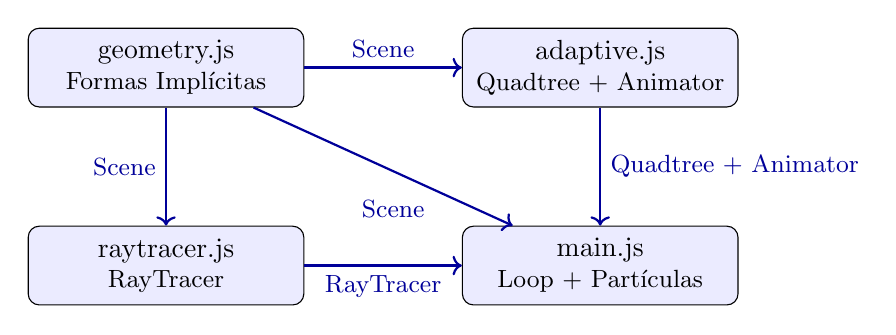
\begin{tikzpicture}[
    node distance=1.2cm,
    box/.style={rectangle, draw, rounded corners, minimum width=3.5cm,
                minimum height=1cm, align=center, fill=blue!8},
    arr/.style={->, thick, blue!60!black}
]
\node[box] (geo)  {\shortstack{geometry.js\\\small Formas Implícitas}};
\node[box, right=2cm of geo] (ada)  {\shortstack{adaptive.js\\\small Quadtree + Animator}};
\node[box, below=1.5cm of geo] (ray)  {\shortstack{raytracer.js\\\small RayTracer}};
\node[box, below=1.5cm of ada] (main) {\shortstack{main.js\\\small Loop + Partículas}};

\draw[arr] (geo) -- (ada)  node[midway, above, font=\small] {Scene};
\draw[arr] (geo) -- (ray)  node[midway, left,  font=\small] {Scene};
\draw[arr] (ada) -- (main) node[midway, right, font=\small] {Quadtree + Animator};
\draw[arr] (ray) -- (main) node[midway, below, font=\small] {RayTracer};
\draw[arr] (geo) -- (main) node[midway, below left, font=\small, pos=0.7] {Scene};
\end{tikzpicture}
\end{center}

\subsection{Sequência de Operações por Frame}

A cada frame do \texttt{requestAnimationFrame}, o loop principal executa:

\begin{enumerate}
    \item \textbf{Leitura dos controles:} atualiza \texttt{lightRange} e
    \texttt{numRays} a partir dos sliders.
    \item \textbf{Renderização do fundo:}
    \begin{itemize}
        \item \emph{Modo Lanterna:} \texttt{RayTracer.renderLight()} lança $N$
        raios e pinta os gradientes de luz.
        \item \emph{Modo Quadtree:} \texttt{AdaptiveQuadtreeAnimator.step()} e
        \texttt{.draw()} revelam progressivamente a estrutura, seguidos da
        sobreposição dos contornos de fronteira.
    \end{itemize}
    \item \textbf{Física de partículas:} para cada partícula, \texttt{update()}
    integra a posição e resolve colisões.
    \item \textbf{Renderização de partículas:} para cada partícula, \texttt{draw()}
    lança o shadow ray e, se visível, pinta o halo e o núcleo.
\end{enumerate}

\subsection{Evento \texttt{rebuild()}}

O evento \texttt{rebuild()} é disparado sempre que a cena muda (adição de forma,
limpeza, mudança de profundidade). Ele:
\begin{enumerate}
    \item Reconstrói a \texttt{Quadtree} do zero com a cena atual.
    \item Chama \texttt{prune()} para otimizar a árvore.
    \item Reinicia o \texttt{AdaptiveQuadtreeAnimator} com a nova árvore.
\end{enumerate}

Isso garante que a Quadtree usada pelo Ray Tracer e pelo Animator é sempre
consistente com a cena em exibição.

% ══════════════════════════════════════════════════════════════════════════════
\section{Funções Customizadas: da String ao Código}
\label{sec:custom}

O sistema permite que o usuário insira uma expressão matemática como string ---
por exemplo, \texttt{"x*x + y*y - 0.25"} --- e a utilize como função implícita.
A transformação ocorre em dois passos:

\textbf{Passo 1: Compilação.} A string é convertida em uma função JavaScript
usando o construtor \texttt{Function}:
\begin{lstlisting}
this.func = new Function('x', 'y', `return ${exprStr};`);
\end{lstlisting}
Isso cria uma função anônima equivalente a \texttt{(x, y) => exprStr}. O motor
V8 do Chrome/Node compila essa função para bytecode nativo, garantindo performance
equivalente a código escrito manualmente.

\textbf{Passo 2: Avaliação no domínio correto.} Cada chamada a
\texttt{evaluate(px, py)} primeiro converte as coordenadas de pixel para o
domínio $[-2, 2]$ (equações \eqref{eq:mapx} e \eqref{eq:mapy}) antes de chamar
\texttt{this.func}.

\begin{example}[Equações que podem ser inseridas]
\begin{itemize}
    \item \texttt{x*x + y*y - 0.25} --- círculo de raio $0.5$ centrado na origem.
    \item \texttt{y - x*x} --- parábola $y = x^2$ (interior abaixo da curva).
    \item \texttt{x*x/0.25 + y*y/1.0 - 1} --- elipse com semi-eixos $a=0.5$, $b=1$.
    \item \texttt{Math.sin(x*3) - y} --- curva senoidal.
    \item \texttt{Math.abs(x) + Math.abs(y) - 0.5} --- quadrado rotacionado 45°
    (losango).
\end{itemize}
\end{example}

% ══════════════════════════════════════════════════════════════════════════════
\section{Conclusão}
\label{sec:conclusao}

Este trabalho demonstrou como conceitos fundamentais de matemática aplicada se
traduzem diretamente em sistemas computacionais funcionais e eficientes:

\begin{itemize}
    \item A \textbf{geometria implícita} fornece o substrato matemático unificado
    que permite descrever formas arbitrárias, testá-las por inclusão em $O(1)$ e
    combiná-las por operações de conjuntos (min/max).

    \item A \textbf{Quadtree adaptativa} é a estrutura de dados que torna o
    sistema escalável: concentra representação e computação na fronteira das
    formas, onde o comportamento é complexo, e descarta regiões uniformes com
    custo constante.

    \item O \textbf{Ray Tracing} combina a elegância do método das lâminas para
    teste AABB com o pragmatismo do raymarching para localizar fronteiras
    implícitas com precisão sub-pixel, tudo acelerado pela hierarquia da Quadtree.

    \item A \textbf{física de partículas} demonstra que o gradiente de uma função
    implícita é não apenas um conceito teórico de análise, mas uma ferramenta
    prática imediata para computar normais e resolver reflexões sem qualquer
    conhecimento explícito da geometria.
\end{itemize}

A integração desses quatro pilares num loop de tempo real --- mantendo 60fps no
navegador com centenas de partículas e centenas de raios --- valida a premissa
central: a modelagem matemática rigorosa não é antagonista do desempenho
computacional, mas sua precondição.

% ══════════════════════════════════════════════════════════════════════════════
\appendix
\section{Pseudocódigo Completo do Loop Principal}

\begin{algorithm}[H]
\caption{Loop Principal de Renderização}
\begin{algorithmic}[1]
\Procedure{Loop}{nowMs}
    \State Atualiza $R \gets$ \texttt{lightRange}, $N \gets$ \texttt{numRays}
    \If{modo = \textsc{Lanterna}}
        \State Pinta fundo preto
        \State $\text{isInside} \gets f_{\text{scene}}(\vv{o}) \leq 0$
        \For{$i = 0$ \textbf{to} $N-1$}
            \State $\theta_i \gets 2\pi i / N$
            \State $\vv{d} \gets (\cos\theta_i, \sin\theta_i)$
            \State \texttt{hit} $\gets$ \Call{Trace}{root, $\vv{o}$, $\vv{d}$, isInside, scene}
            \State $t_{\text{end}} \gets \min(\text{hit.t se hit}, R)$
            \State Pinta gradiente de $\vv{o}$ até $\vv{o} + t_{\text{end}} \vv{d}$
        \EndFor
    \Else \Comment{Modo Quadtree}
        \State \Call{AnimatorStep}{nowMs}
        \State \Call{AnimatorDraw}{ctx}
        \State Sobrepõe contornos de nós Status 2
    \EndIf
    \For{cada partícula $p$}
        \State \Call{Update}{$p$, scene}
        \State \Call{DrawParticle}{$p$, $\vv{o}$, R, scene, quadtree}
    \EndFor
    \State \textbf{requestAnimationFrame}(\Call{Loop}{})
\EndProcedure
\end{algorithmic}
\end{algorithm}

\section{Tabela de Parâmetros do Sistema}

\begin{center}
\begin{tabular}{llll}
\toprule
\textbf{Parâmetro} & \textbf{Símbolo} & \textbf{Padrão} & \textbf{Intervalo} \\
\midrule
Número de raios          & $N$           & 720   & [90, 1440]  \\
Profundidade da Quadtree & $d_{\max}$    & 7     & [2, 10]     \\
Alcance da lanterna      & $R$           & 300px & [50, 600]px \\
Expoente de decaimento   & $\alpha$      & 2.5   & (fixo)      \\
Raio do círculo padrão   & $r$           & 0.08  & (fixo)      \\
Passo do raymarching     & $\Delta t$    & 1.0px & (fixo)      \\
Passo do gradiente       & $\eps$        & 1.0px & (fixo)      \\
Velocidade da partícula  & $\norm{\vv{v}}$ & $\sim$4.2px/frame & (aleatório) \\
\bottomrule
\end{tabular}
\end{center}

\begin{thebibliography}{99}

\bibitem{chalmers}
GOMES, Jonas; VELHO, Luiz.: \textbf{Fundamentos da Computação Gráfica} (Foco em modelagem geométrica e síntase de imagem).

\bibitem{shirley}
SHIRLEY, Peter; MARSHNER, Steve.: \textbf{Fundamentals of Computer Graphics}. A. K. Peters/CRC Press, (Referência para fundamentação de Ray Tracing).

\bibitem{preparata}
PREPARATA, F. P; SHAMOS, M I. (1985).: \textbf{Computational Geometry: An Introduction"}. Springer-Verlag

\bibitem{samet}
SAMET, H. (1984) \textbf{The Quadtree and Related Hierarchical Data Structures}. ACM Computing Surveys

\bibitem{pharr}
PHARR, Matt:, JAKOB. Wenzel; HUMPHREYS. Greg \textbf{Physically Based Rendering: From Theory To Implementation. } Morgan Kaufmann. (Teoria avançada de modelagem para transporte de luz).

\bibitem{visgraf2026}
VISGRAF Lab. \textbf{Topologia e Computação Visual 2026}. Disponível em: <https://visgraf.github.io/tcv-2026/>. Acesso em: 14 mai. 2026.

\end{thebibliography}



\end{document}